\documentclass{beamer}
\usepackage[backend=bibtex,style=numeric,sorting=none]{biblatex}
\usepackage{progressbar}
\usepackage[final]{listings}
\usepackage{graphicx}
\usepackage{wrapfig}
\usepackage{tikz}
\usepackage{tcolorbox}
\usepackage{hyperref}
\usepackage{CJKutf8}
\graphicspath{ {./images/} }

\usepackage{caption}
\captionsetup{justification   = raggedright,
              singlelinecheck = false}

\addbibresource{main.bib}
\usetheme{AnnArbor}

\title{The Container Security in Healthcare Data Exchange System}
\subtitle{Bachelor's degree graduation project}
\author{Chih-Hsuan Yang}
\institute{National Sun Yat-sen University}
\date{\today\\v1.0}

\AtBeginSection[]{
    \begin{frame}
        \vfill
        \centering
        \begin{beamercolorbox}[sep=8pt,center,shadow=true,rounded=true]{title}
          \usebeamerfont{title}\insertsectionhead\par
        \end{beamercolorbox}
        \vfill
        \end{frame}
}

\definecolor{mygreen}{rgb}{0,0.6,0}
\definecolor{mygray}{rgb}{0.5,0.5,0.5}
\definecolor{mymauve}{rgb}{0.58,0,0.82}
\definecolor{tiffanyblue}{rgb}{0.04, 0.73, 0.71}

% Code conf.
\lstset{ 
  backgroundcolor=\color{white},   % choose the background color; you must add \usepackage{color} or \usepackage{xcolor}; should come as last argument
  basicstyle=\ttfamily\footnotesize,% the size of the fonts that are used for the code
  breakatwhitespace=false,         % sets if automatic breaks should only happen at whitespace
  breaklines=true,                 % sets automatic line breaking
  captionpos=b,                    % sets the caption-position to bottom
  commentstyle=\color{mygreen},    % comment style
  deletekeywords={...},            % if you want to delete keywords from the given language
  escapeinside={\%*}{*)},          % if you want to add LaTeX within your code
  extendedchars=true,              % lets you use non-ASCII characters; for 8-bits encodings only, does not work with UTF-8
  frame=single,	                   % adds a frame around the code
  keepspaces=true,                 % keeps spaces in text, useful for keeping indentation of code (possibly needs columns=flexible)
  keywordstyle=\color{red},       % keyword style
  morekeywords={*,...},            % if you want to add more keywords to the set
  numbers=left,                    % where to put the line-numbers; possible values are (none, left, right)
  numbersep=5pt,                   % how far the line-numbers are from the code
  numberstyle=\tiny\color{mygray}, % the style that is used for the line-numbers
  rulecolor=\color{black},         % if not set, the frame-color may be changed on line-breaks within not-black text (e.g. comments (green here))
  showspaces=false,                % show spaces everywhere adding particular underscores; it overrides 'showstringspaces'
  showstringspaces=false,          % underline spaces within strings only
  showtabs=false,                  % show tabs within strings adding particular underscores
  stepnumber=1,                    % the step between two line-numbers. If it's 1, each line will be numbered
  stringstyle=\color{mymauve},     % string literal style
  tabsize=4,	                     % sets default tabsize to ˋ spaces
}


\begin{document}
\begin{CJK*}{UTF8}{bsmi}

    \begin{frame}
        \titlepage
    \end{frame}

    \begin{frame}
        \frametitle{Outline}
        \tableofcontents
    \end{frame}

    % ======================Outcome============================
    \section{Outcome}
    \begin{frame}
        \frametitle{Outcome}
        \centering \Large {Zombie escalation not works?}
    \end{frame}


    % ======================Related works============================

    \section{Related works}
    \begin{frame}{Document\&Patter}
        \begin{enumerate}
            \item \url{https://www.usenix.org/sites/default/files/conference/protected-files/ucms15_slides_vantuin.pdf}
            \item \url{https://blog.phusion.nl/2015/01/20/docker-and-the-pid-1-zombie-reaping-problem/}
            \item \url{https://blog.phusion.nl/2015/01/20/baseimage-docker-fat-containers-treating-containers-vms/}
        \end{enumerate}


        ToDo:
        \begin{enumerate}
            \item\url{https://www.usenix.org/conference/usenixsecurity20/presentation/xiong}
        \end{enumerate}

    \end{frame}
    \begin{frame}{Containter escalation}
        \centering\Large{Zombie escalation}
    \end{frame}

    \begin{frame}{picosh}
        \lstinputlisting[xleftmargin=1em, language=C, linerange={122,134}, firstnumber=122]{src/picosh.c}
    \end{frame}

    \begin{frame}{End of file}
        \lstinputlisting[basicstyle=\scriptsize, xleftmargin=1em, language=C, linerange={87-97,99-103,110-113}, firstnumber=87]{src/picosh.c}
    \end{frame}

    \begin{frame}{chroot}
        \centering\Large{chroot jail break.}
    \end{frame}

    \begin{frame}{jb.c}
        \lstinputlisting[basicstyle=\scriptsize, xleftmargin=1em, language=C]{src/chroot/jb.c}
    \end{frame}

    \begin{frame}{Demo}
        \centering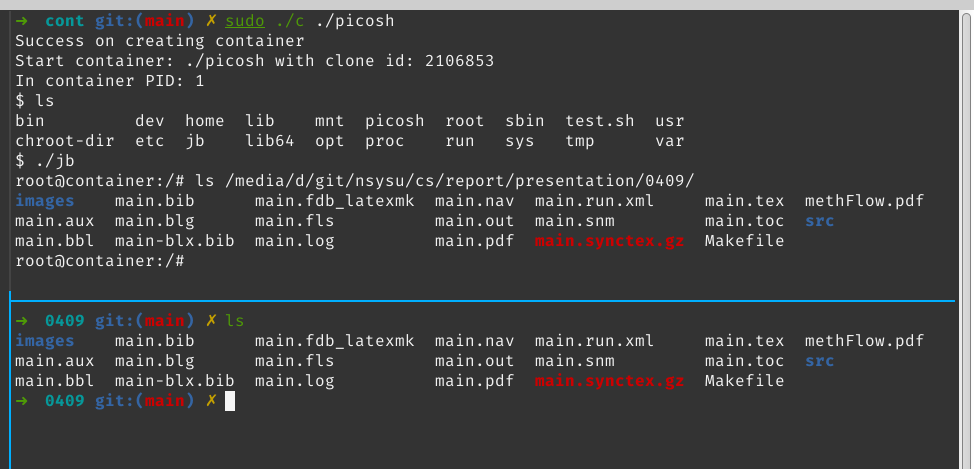
\includegraphics[width=\textwidth]{Screenshot_2021-04-09_09-44-40.png}
    \end{frame}

    \begin{frame}{Swiss cheese model}
        \centering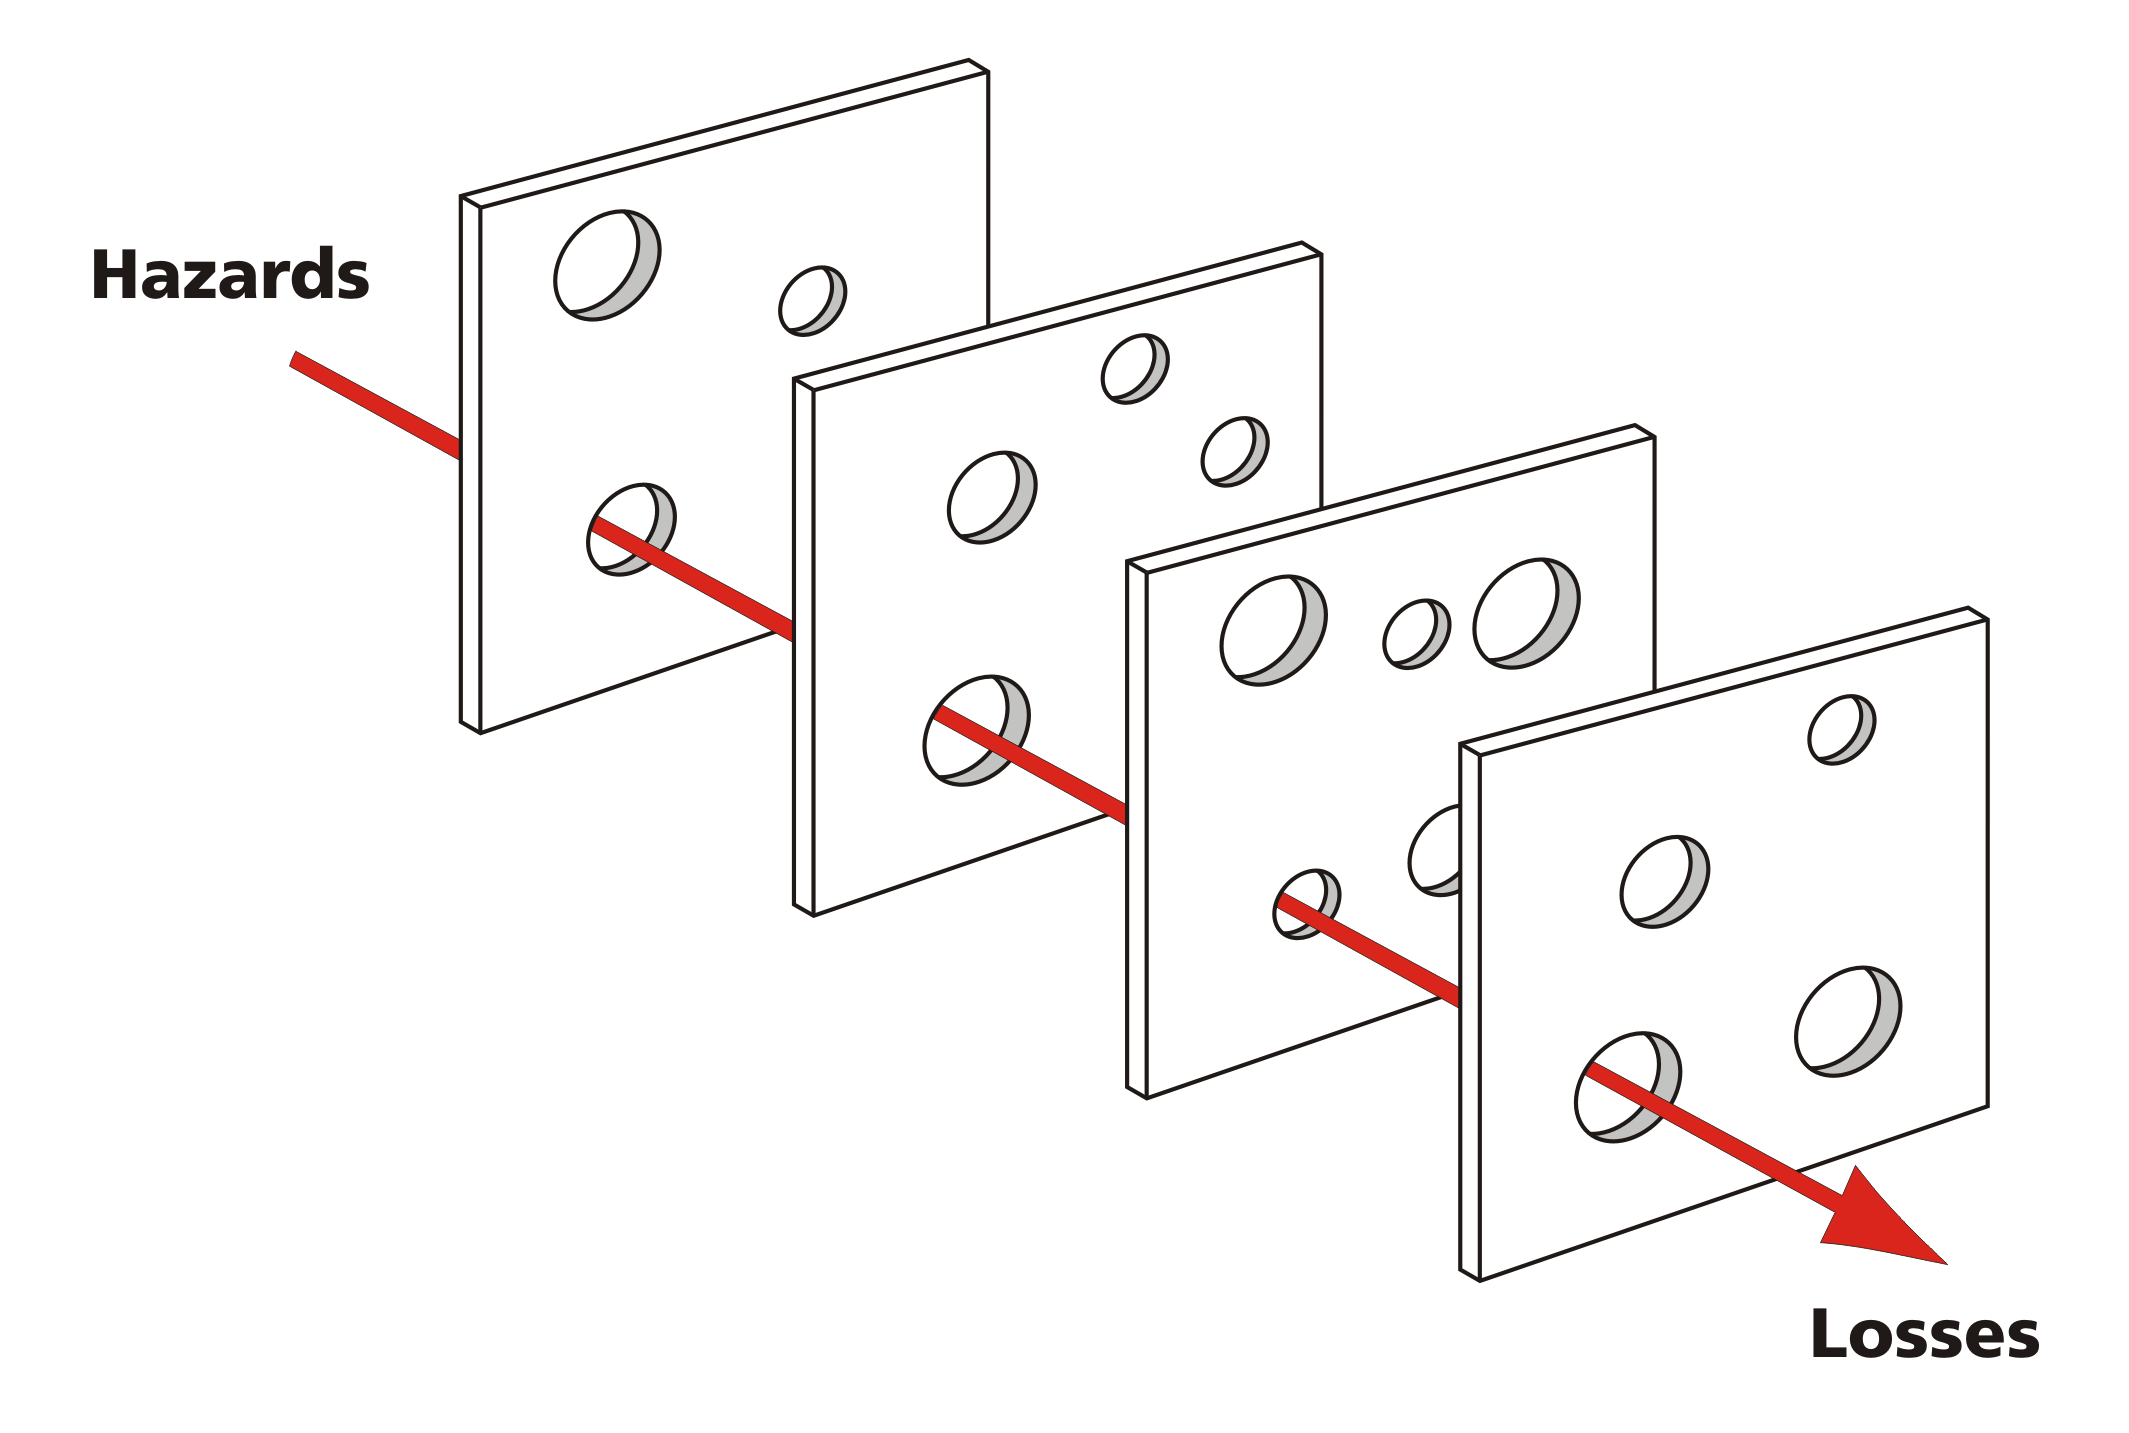
\includegraphics[width=.8\textwidth]{Swiss_cheese_model_of_accident_causation.png}
        \url{https://www.wikiwand.com/en/Swiss_cheese_model}
    \end{frame}

    \begin{frame}{Conditions}
        \begin{enumerate}
            \item Root privileges
            \item Pre-compiled or has a compiler
            \item \textcolor{tiffanyblue}{Task structure}
        \end{enumerate}
    \end{frame}

    % ======================Current progress============================

    \section{Current progress}
    \begin{frame}
        \frametitle{Map-reduce}
        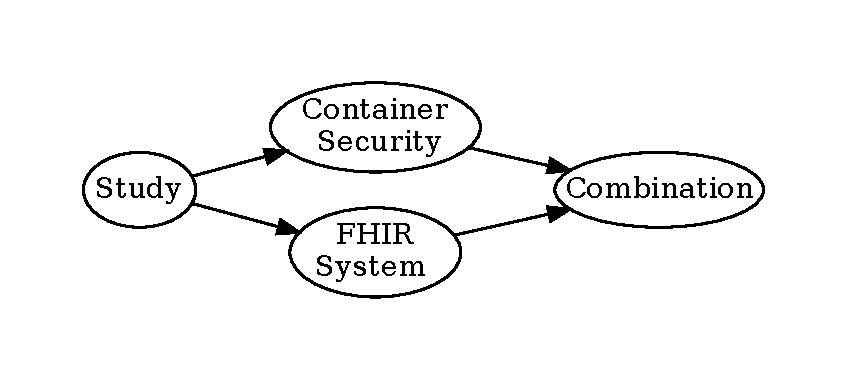
\includegraphics[width=\textwidth]{methFlow.pdf}
    \end{frame}

    \begin{frame}
        \frametitle{Map-reduce}
        \begin{itemize}
            \item \makebox[3cm]{Study: \hfill} \progressbar[width=4cm,heightr=1,filledcolor=red,
                      emptycolor=blue!30]{0} $\frac{12}{\infty}$
            \item \makebox[3cm]{Container Security: \hfill} \progressbar[width=4cm,heightr=1,filledcolor=red,
                      emptycolor=blue!30]{0} read some
            \item \makebox[3cm]{FHIR system: \hfill} \progressbar[width=4cm,heightr=1,filledcolor=red,
                      emptycolor=blue!30]{0} Configured, can run.
            \item \makebox[3cm]{Combination: \hfill} \progressbar[width=4cm,heightr=1,filledcolor=red,
                      emptycolor=blue!30]{0} Of course: 0
            \item \makebox[3cm]{專題競賽暨成果展: \hfill} \progressbar[width=4cm,heightr=1,filledcolor=red,
                      emptycolor=blue!30]{0.241509433962} $\frac{64}{265} \sim 0.2415$
        \end{itemize}
    \end{frame}

    % \section{Reference}
    % \begin{frame}[t, allowframebreaks]
    %     \frametitle{References}
    %     \setbeamertemplate{bibliography item}{\insertbiblabel}
    %     \renewcommand*{\bibfont}{\scriptsize}
    %     \printbibliography
    % \end{frame}

\end{CJK*}
\end{document}